\documentclass{article}
\usepackage{fullpage}
\usepackage[utf8]{inputenc}
\usepackage{pict2e}
\usepackage{amsmath}
\usepackage{enumitem}
\usepackage{eurosym}
\usepackage{mathtools}
\usepackage{amssymb, amsfonts, latexsym, cancel}
\setlength{\parskip}{0.3cm}
\usepackage{graphicx}
\usepackage{fontenc}
\usepackage{slashbox}
\usepackage{setspace}
\usepackage{gensymb}
\usepackage{accents}
\usepackage{adjustbox}
\setstretch{1.35}
\usepackage{bold-extra}
\usepackage[document]{ragged2e}
\usepackage{subcaption}
\usepackage{tcolorbox}
\usepackage{xcolor, colortbl}
\usepackage{wrapfig}
\usepackage{empheq}
\usepackage{array}
\usepackage{parskip}
\usepackage{arydshln}
\graphicspath{ {images/} }
\renewcommand*\contentsname{\color{black}Índice} 
\usepackage{array, multirow, multicol}
\definecolor{lightblue}{HTML}{007AFF}
\usepackage{color}
\usepackage{etoolbox}
\usepackage{listings}
\usepackage{mdframed}
\setlength{\parindent}{0pt}
\usepackage{underscore}
\usepackage{hyperref}
\usepackage{tikz}
\usepackage{tikz-cd}
\usetikzlibrary{shapes, positioning, patterns}
\usepackage{tikz-qtree}
\usepackage{biblatex}
\usepackage{pdfpages}
\usepackage{pgfplots}
\usepackage{pgfkeys}
\addbibresource{biblatex-examples.bib}
\usepackage[a4paper, left=1cm, right=1cm, top=1cm,
bottom=1.5cm]{geometry}
\usepackage{titlesec}
\usepackage{titletoc}
\usepackage{tikz-3dplot}
\usepackage{kbordermatrix}
\usetikzlibrary{decorations.pathreplacing}
\newcommand{\Ej}{\textcolor{lightblue}{\underline{Ejemplo}}}
\setlength{\fboxrule}{1.5pt}

% Configura el formato de las secciones utilizando titlesec
\titleformat{\section}
{\color{red}\normalfont\LARGE\bfseries}
{Tema \thesection:}
{10 pt}
{}

% Ajusta el formato de las entradas de la tabla de contenidos
\addtocontents{toc}{\protect\setcounter{tocdepth}{4}}
\addtocontents{toc}{\color{black}}

\titleformat{\subsection}
{\normalfont\Large\bfseries\color{red}}{\thesubsection)}{1em}{\color{lightblue}}

\titleformat{\subsubsection}
{\normalfont\large\bfseries\color{red}}{\thesubsubsection)}{1em}{\color{lightblue}}

\newcommand{\bboxed}[1]{\fcolorbox{lightblue}{lightblue!10}{$#1$}}
\newcommand{\rboxed}[1]{\fcolorbox{red}{red!10}{$#1$}}

\DeclareMathOperator{\N}{\mathbb{N}}
\DeclareMathOperator{\Z}{\mathbb{Z}}
\DeclareMathOperator{\R}{\mathbb{R}}
\DeclareMathOperator{\Q}{\mathbb{Q}}
\DeclareMathOperator{\K}{\mathbb{K}}
\DeclareMathOperator{\im}{\imath}
\DeclareMathOperator{\jm}{\jmath}
\DeclareMathOperator{\col}{\mathrm{Col}}
\DeclareMathOperator{\fil}{\mathrm{Fil}}
\DeclareMathOperator{\rg}{\mathrm{rg}}
\DeclareMathOperator{\nuc}{\mathrm{nuc}}
\DeclareMathOperator{\dimf}{\mathrm{dimFil}}
\DeclareMathOperator{\dimc}{\mathrm{dimCol}}
\DeclareMathOperator{\dimn}{\mathrm{dimnuc}}
\DeclareMathOperator{\dimr}{\mathrm{dimrg}}
\DeclareMathOperator{\dom}{\mathrm{Dom}}
\DeclareMathOperator{\infi}{\int_{-\infty}^{+\infty}}
\newcommand{\dint}[2]{\int_{#1}^{#2}}

\newcommand{\bu}[1]{\textcolor{lightblue}{\underline{#1}}}
\newcommand{\lb}[1]{\textcolor{lightblue}{#1}}
\newcommand{\db}[1]{\textcolor{blue}{#1}}
\newcommand{\rc}[1]{\textcolor{red}{#1}}
\newcommand{\tr}{^\intercal}

\renewcommand{\CancelColor}{\color{lightblue}}

\newcommand{\dx}{\:\mathrm{d}x}
\newcommand{\dt}{\:\mathrm{d}t}
\newcommand{\dy}{\:\mathrm{d}y}
\newcommand{\dz}{\:\mathrm{d}z}
\newcommand{\dth}{\:\mathrm{d}\theta}
\newcommand{\dr}{\:\mathrm{d}\rho}
\newcommand{\du}{\:\mathrm{d}u}
\newcommand{\dv}{\:\mathrm{d}v}
\newcommand{\tozero}[1]{\cancelto{0}{#1}}
\newcommand{\lbb}[2]{\textcolor{lightblue}{\underbracket[1pt]{\textcolor{black}{#1}}_{#2}}}
\newcommand{\dbb}[2]{\textcolor{blue}{\underbracket[1pt]{\textcolor{black}{#1}}_{#2}}}
\newcommand{\rub}[2]{\textcolor{red}{\underbracket[1pt]{\textcolor{black}{#1}}_{#2}}}

\author{Francisco Javier Mercader Martínez}
\date{}
\title{Procesos Estocásticos y Series Temporales}
\usepackage{amsthm}
\theoremstyle{definition}
\newtheorem{definition}{Definición}[section]
\usepackage{framed}
\newenvironment{knitrout}{}{}
\newcolumntype{C}[1]{>{\centering\arraybackslash}p{#1}}
% Colores que knitr suele referenciar
\definecolor{fgcolor}{rgb}{0.345,0.345,0.345}
\definecolor{shadecolor}{rgb}{0.97,0.97,0.97}

\begin{document}
\maketitle
\tableofcontents
\newpage
\section{Introducción a los procesos estocásticos}
Los procesos estocásticos modelizan cantidades numéricas que cambian con el tiempo de manera aleatoria. Ejemplos del mundo real de estos procesos incluyen:
\begin{enumerate}
    \item Resultados sucesivos en un juego de azar.
    \item Número de plazas ocupadas en un parking.
    \item Porcentaje de cielo cubierto en el cielo de Madrid.
    \item Evolución del precio de activos financieros: acciones, tipos de cambio de divisas o criptomonedas, materias primas, etc.
    \item Indicadores económicos como la inflación, el precio de la luz, y el IBEX 35.
\end{enumerate}
Los procesos estocásticos proporcionan marcos matemáticos para modelar y comprender estos fenómenos, lo que permite hacer predicciones y tomar decisiones informadas.

\begin{figure}[h]
\begin{knitrout}
\definecolor{shadecolor}{rgb}{0.969, 0.969, 0.969}\color{fgcolor}

{\centering 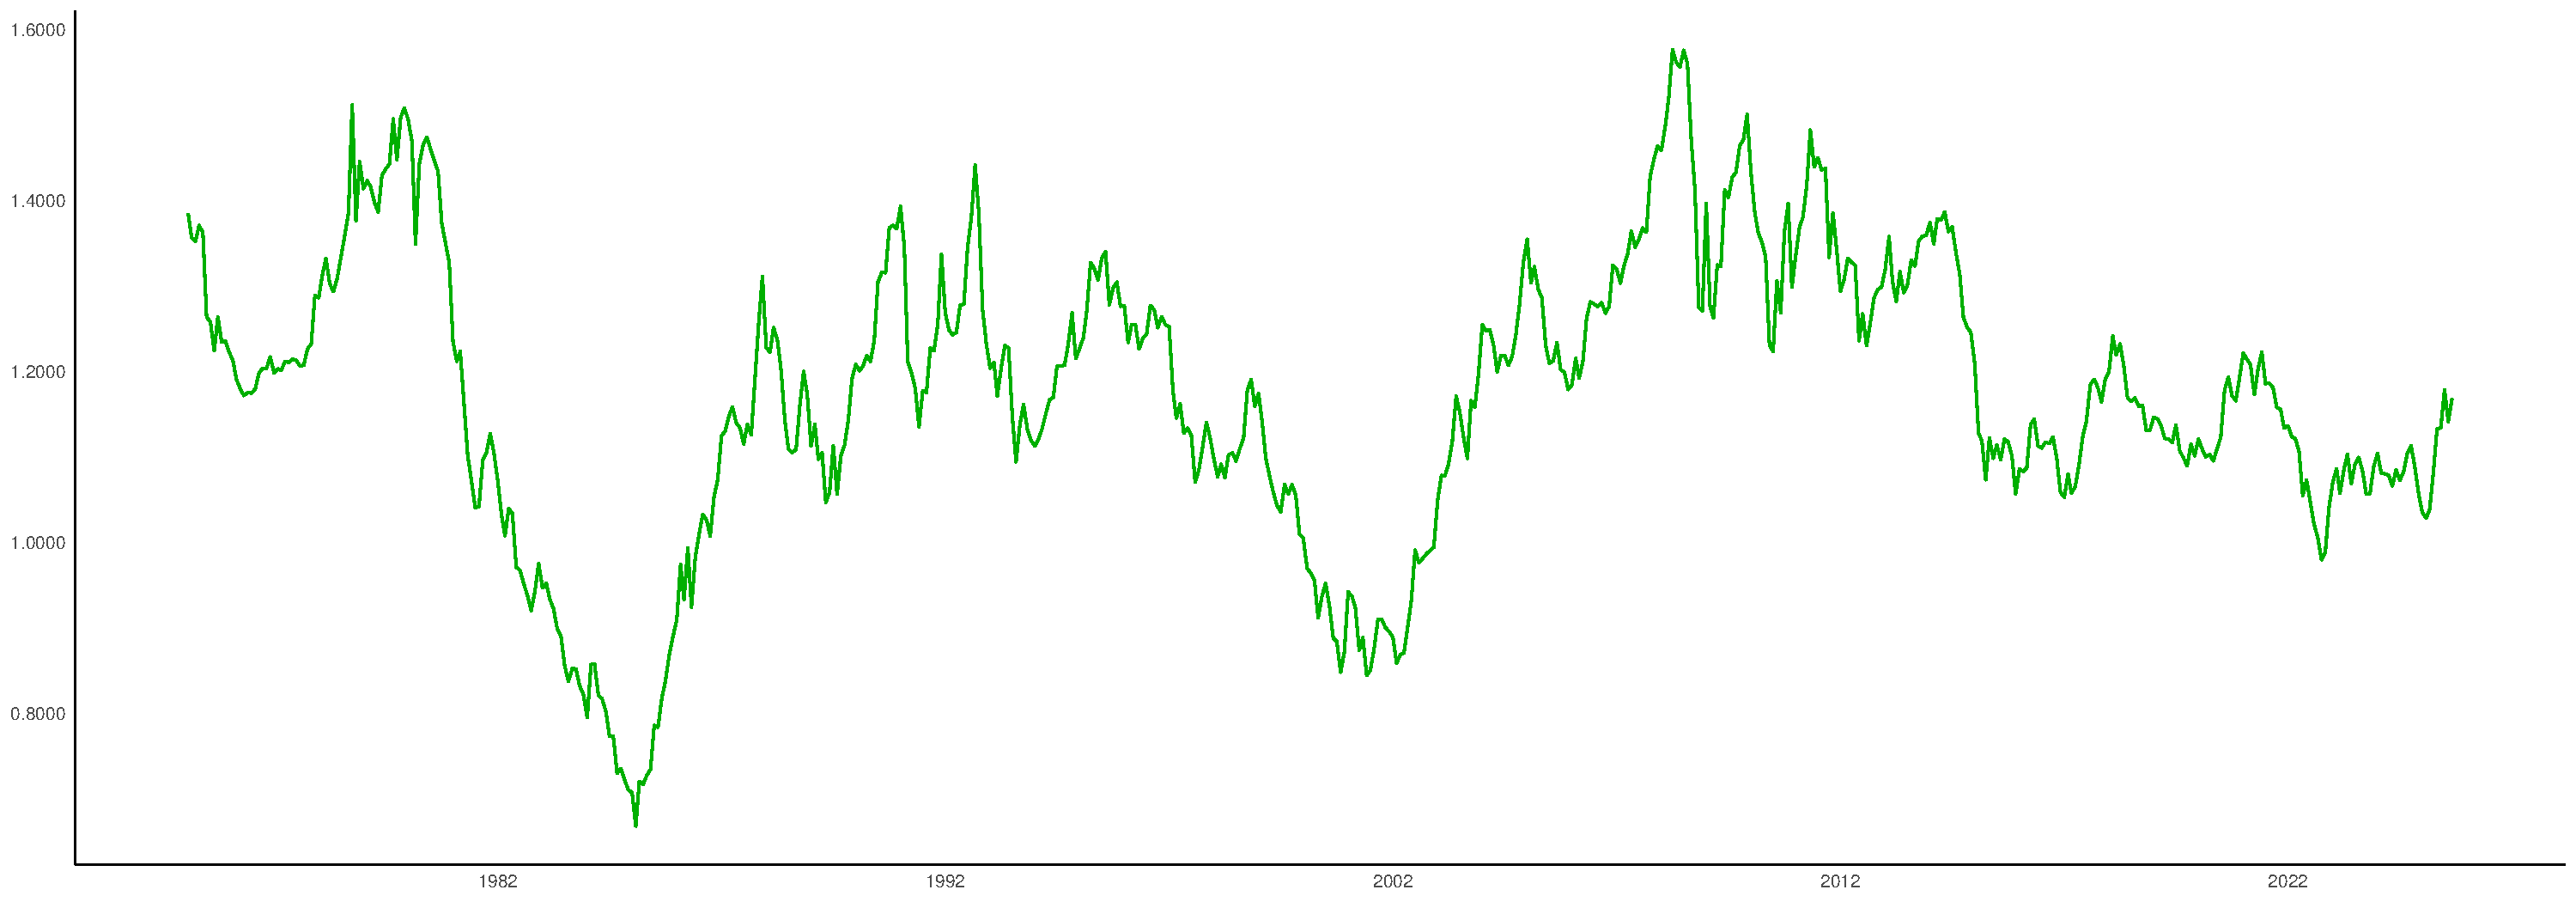
\includegraphics[width=0.7\textwidth]{figure/unnamed-chunk-1-1} 

}


\end{knitrout}
\caption{Evolución del tipo de cambio Euro/dolar (Fuente: Google Finance)}
\end{figure}
\subsection{Concepto de proceso estocástico, trayectorias y ejemplos}
A lo largo de este tema, vamos a fijar un espacio de probabilidad $(\Omega, \mathcal{F}, \mathbb{P})$ y un subconjunto $\mathbb{T}\subset[0,\infty)$.
\begin{definition}
    Un \textbf{proceso estocástico} $(X_t)_{t\in \mathbb{T}}$ es una colección de variables aleatorias reales $X_t$ definidas en el espacio de probabilidad  $(\Omega, \mathcal{F}, \mathbb{P})$.
\end{definition}
Interpretamos $t$ como el tiempo (medido en cierta unidad).
 \begin{itemize}[label=\textbullet]
    \item Si $\mathbb{T}$ es contable (por ejemplo, $\mathbb{T}=\{0<1<2<\dots\} $), diremos que el proceso estocástico $(X_t)_{t\in \mathbb{T}}$ es de tiempo discreto.
    \item Si $\mathbb{T}$ es un intervalo (por ejemplo, $\mathbb{T}=[0,T]$ o $\mathbb{T}=[0,\infty)$), diremos que el proceso estocástico es de tiempo continuo.
\end{itemize}
Para cada $t\in \mathbb{T}$ tenemos una variable aleatoria $X_t$. La variable aleatoria  $X_t$ tomará un valor numérico  $X_t(\omega)$ para cada $\omega\in \Omega$. A los posibles valores que toma un proceso estocástico se les llama \textbf{estados}. 
\begin{itemize}[label=\textbullet]
    \item Si para cada $t\in \mathbb{T}$ la variable aleatoria $X_t$ es de tipo discreto, diremos que el proceso estocástico  $(X_t)_{t\in \mathbb{T}}$ es de estado discreto.
    \item Si para cada $t\in \mathbb{T}$ la variable aleatoria $X_t$ es de tipo continuo, diremos que el proceso estocástico  $(X_t)_{t\in \mathbb{T}}$ es de estado continuo.
\end{itemize}
\newpage
\begin{figure}[h]
    \centering
    \begin{tabular}{|m{2.5cm}|m{4cm}|m{4cm}|}
        \hline
         & $t$ \textbf{Discreto} & $t$  \textbf{Continuo} \\ \hline
    $X$ \textbf{Discreta} & Proceso de estado discreto y tiempo discreto (Unidades prod. mensualmente de un producto) & Proceso de estado discreto y tiempo continuo (Unidades producidas hasta $t$) \\ \hline
$X$ \textbf{Continua} & Proceso de estado continuo y tiempo discreto (Toneladas de producción diaria de un producto) & Proceso de estado continuo y tiempo continuo (Velocidad de un vehículo en el instante $t$) \\ \hline
    \end{tabular}
    \caption{Tipos de procesos estocásticos}
\end{figure}

En lo que sigue, siempre supondremos que $0\in \mathbb{T}$. Esta condición no es realmente restrictiva, ya que podemos desplazar el tiempo por una constante para garantizar que dicha condición se cumple.
\subsection{Procesos gaussianos}
\begin{definition}
   Diremos que un proceso estocástico $(X_t)_{t\in T}$ es gaussiano si que cualquier colección de índices temporales $t_1,t_2,\dots,t_n \in T$, el vector aleatorio $(X_{t_1}, X_{t_2},\dots,X_{t_n})$ sigue un \textbf{Normal multivariante}.
\end{definition}
\newpage
\begin{center}
    \textbf{\Large Hoja 1: Problemas de Introducción a los Procesos Estocásticos} 
\end{center}
\begin{enumerate}[label=\color{red}\textbf{\arabic*)}]
    \item \lb{¿Qué es un proceso estocástico y cómo se define formalmente?}
    \item \lb{¿Cuáles son los tipos principales de procesos estocásticos en función del tiempo?}
    \item \lb{¿Cómo se clasifica un proceso estocástico según los estados que puede formar?} 
\end{enumerate}
\end{document}
